\documentclass[12pt,a4paper]{article}

\usepackage[utf8]{inputenc}
\usepackage[T2A]{fontenc}
\usepackage[ukrainian]{babel}

\usepackage{geometry}
\geometry{left=2cm,right=2cm,top=2cm,bottom=2cm}

\usepackage{graphicx}
\usepackage{array,multirow}
\usepackage{booktabs}
\usepackage{caption}
\renewcommand{\thetable}{\arabic{table}}
\captionsetup[table]{name=Таблиця}

\usepackage{amsmath}
\usepackage{pdflscape}
\usepackage{xcolor}

\usepackage{hyperref}

\begin{document}

    \begin{titlepage}

        % Картинка шапки (по центру, з відступом від верху)
        \begin{center}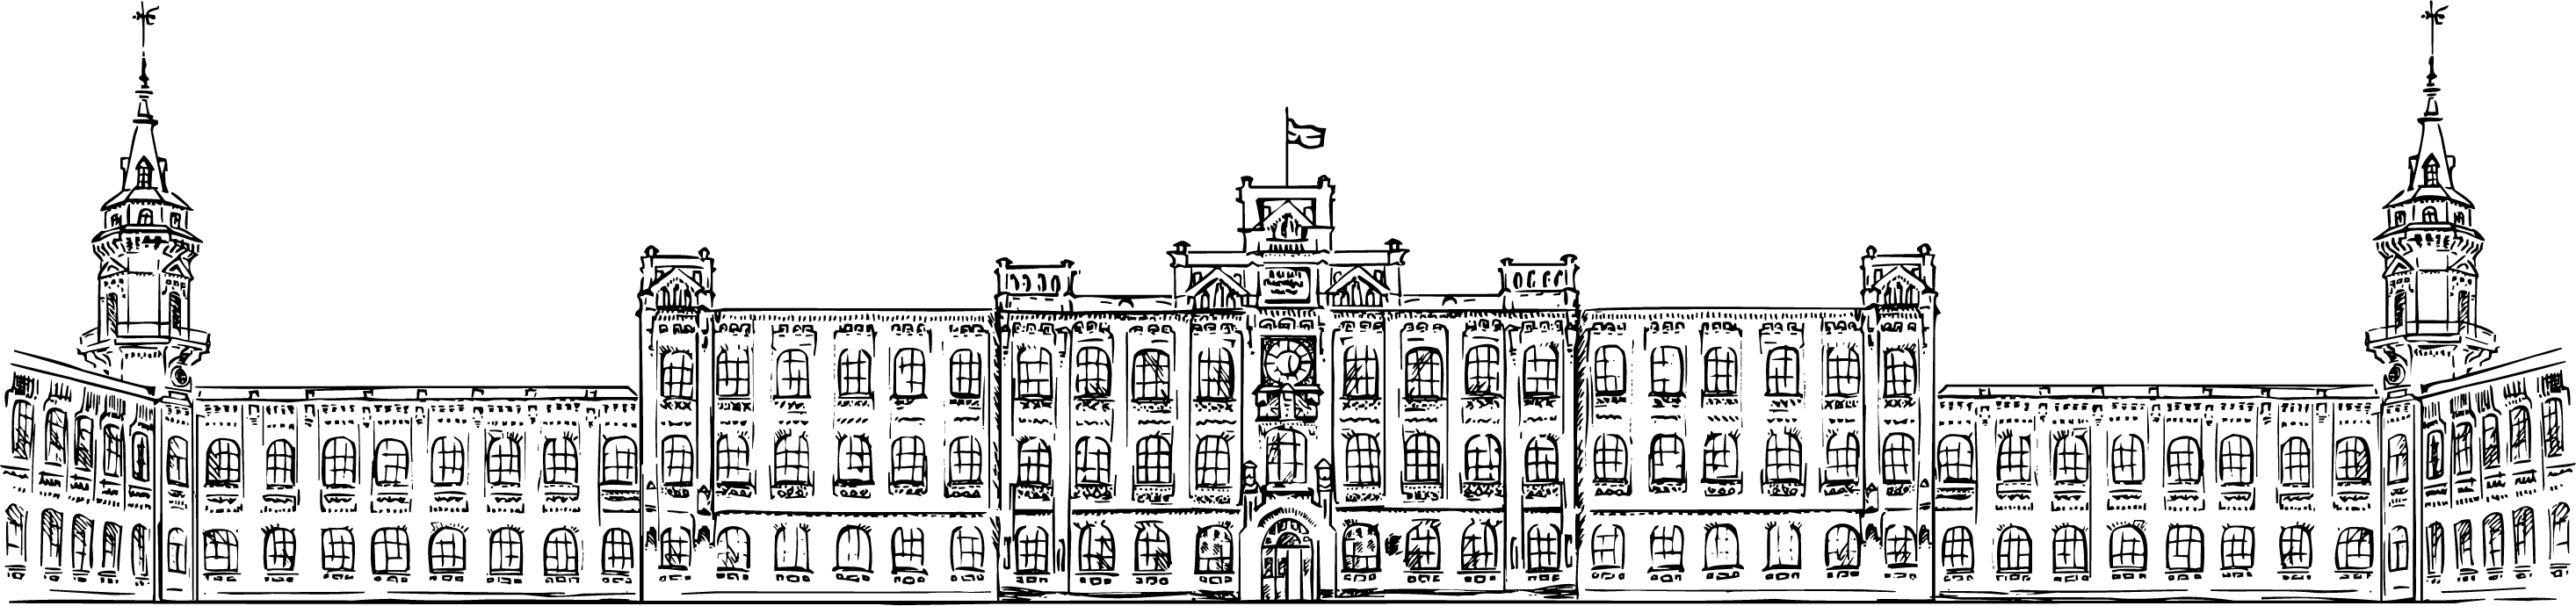
\includegraphics[width=0.7\textwidth]{letterhead.png}\end{center}

        \begin{center}
            \large Національний технічний університет України\\
            «Київський політехнічний інститут імені Ігоря Сікорського»\\[1em]
            Факультет інформатики та обчислювальної техніки\\
            Кафедра обчислювальної техніки
        \end{center}

        \vfill

        \begin{center}
            \textbf{\LARGE Теорія електричних кіл та сигналів}\\[2em]
            \textbf{\Large Лабораторна робота №1}\\
            «Експериментальна перевірка законів Ома та Кірхгофа»
        \end{center}

        \vfill

        \begin{flushright}
            Виконав: студент 2 курсу ФІОТ, гр. ІО-41\\
            \textit{Давидчук А.~М.}\\[1em]
            Перевірив: \textit{Лободзинський В.~Ю.}
        \end{flushright}

        \vfill

        \begin{center}Київ --- 2025\end{center}

    \end{titlepage}

    \setlength{\parindent}{0pt}

    \textbf{\underline{Тема:}} «Експериментальна перевірка законів Ома та Кірхгофа».

    \vspace{1em}

    \textbf{\underline{Мета:}} Навчитися моделювати електричні кола постійного струму.
    Перевірити справедливість основних законів електротехніки – законів Ома і Кірхгофа.

    \begin{center} \textbf{\large Практична частина} \end{center}

    \setlength{\parindent}{1.5em}

    Моя група: ІО-41, мій порядковий номер у групі: 6. Звідси $N = 6$, $S = 1$. Звідси загальна стуктурна схема електричного кола:
    \begin{figure}[h!]

        \renewcommand{\thefigure}{\arabic{figure}} % робимо "3.1", "3.2" і т.д.

        \centering
        % Підставляєте потрібний шлях та розмір зображення:
        
\includegraphics[width=0.3\textwidth]{image1.png}
        % Підпис (зазвичай під малюнком):
        \caption{}
        % Мітка для посилань у тексті (\ref{fig:...})
        \label{fig1:schema}

    \end{figure}

    Відповідно до Таблиці~1 з методичних вказівок, для $N=6$ отримуємо такі елементи у вітках (зведені у Таблиці~1):

    \begin{table}[h!]
        \centering
        \begin{tabular}{|c|c|c|c|c|c|c|}
            \hline
            Варіант & Вітка 1 & Вітка 2 & Вітка 3 & Вітка 4 & Вітка 5 & Вітка 6 \\ \hline
            6 & $R$ & $R$ & $E, R$ & $R$ & $E$ & $R$ \\ \hline
        \end{tabular}
        \caption{Елементи віток для варіанта $N=6$}
        \label{tab:myN6}
    \end{table}

    На основі елементів віток із Таблиці 1 та структурної схеми Рис. 1, побудуємо схему заміщення:
    \begin{figure}[h!]

        \renewcommand{\thefigure}{\arabic{figure}} % робимо "3.1", "3.2" і т.д.

        \centering
        % Підставляєте потрібний шлях та розмір зображення:
        \includegraphics[width=0.8\textwidth]{Figure_1.pdf}
        % Підпис (зазвичай під малюнком):
        \caption{Схема заміщення}
        % Мітка для посилань у тексті (\ref{fig:...})
        \label{fig2:schema}

    \end{figure}

    Відповідно до формул обчислення ЕРС $E_1$ та $E_2$, а також опорів $R_1$, $R_2$, $R_3$, $R_4$, $R_5$, $R_6$,
    що приведені в Таблиці 2 з методичних вказівок, отримуємо:

    \[
    E_1 = N \cdot 10, \text{В} = 60 \,\text{В}
    \]
    \[
    E_2 = N \cdot 5, \text{В} = 30 \,\text{В}
    \]
    \[
    R_1 = 50 + N \cdot S, \text{Ом} = 56 \,\text{Ом}
    \]
    \[
    R_2 = 75 + N \cdot S, \text{Ом} = 81 \,\text{Ом}
    \]
    \[
    R_3 = 120 + N \cdot S, \text{Ом} = 126 \,\text{Ом}
    \]
    \[
    R_4 = 180 + N \cdot S, \text{Ом} = 186 \,\text{Ом}
    \]
    \[
    R_5 = 200 + N \cdot S, \text{Ом} = 206 \,\text{Ом}
    \]
    \[
    R_6 = 220 + N \cdot S, \text{Ом} = 226 \,\text{Ом}
    \]

    І зводимо до зручного вигляду у таблиці:

    \begin{table}[h!]
        \centering
        \begin{tabular}{|c|c|c|c|c|c|c|c|}
            \hline
            $E_1, \text{В}$ & $E_2, \text{В}$ & $R_1, \text{Ом}$ & $R_2, \text{Ом}$ & $R_3, \text{Ом}$ & $R_4, \text{Ом}$ & $R_5, \text{Ом}$ & $R_6, \text{Ом}$ \\ \hline
            60 & 30 & 56 & 81 & 126 & 186 & 206 & 226\\ \hline
        \end{tabular}
        \caption{Розрахункові параметри ел. кола}
    \end{table}







    $R_5$ -- не існує для моєї схеми.

\end{document}